\worksheet{Moneyball Analytics}

The Pythagorean expectation from the chapter says 
\[ P = \frac{RS^2}{RS^2+RA^2}\]
where $RS$ is runs scored, \(RA\) is runs allowed, and \(P\) is the percent of games the team is expected to have won. While the book says that the Pythagorean expectation is loosely connected to the Pythagorean Theorem, \(a^2+b^2=c^2\), \(P\) is more closely aligned to trig functions and could be considered the \(\sin^2(\theta)\) of the following triangle:

\begin{center}
	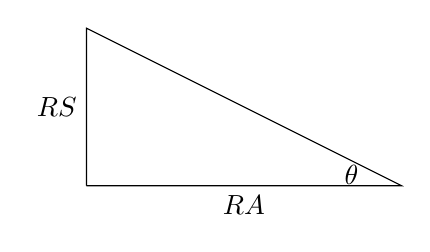
\begin{tikzpicture}
		\draw (0,0) -- node[below, pos=0.5] {\(RA\)} (4,0) node[shift={(-18pt,4pt)}] {\(\theta\)} -- (0,2) -- node[left, pos=0.5] {\(RS\)} (0,0);
	\end{tikzpicture}
\end{center}

\textbf{Worksheet: Compute Like Bill James}

\noindent Test James' Pythagorean expectation for another team. Pick a year and a Major League Baseball Team. Everyone gets a unique team/year.

\begin{enumerate}
	\item Find \emph{runs scored} by your team (RS): \underline{\hspace{2cm}}
	\item Find \emph{runs allowed} by your team (RA): \underline{\hspace{2cm}}
	\item Compute \( P = \frac{RS^2}{RS^2+RA^2}\): \underline{\hspace{2cm}}
	\item Compute \(P\times 162\): \underline{\hspace{2cm}}
\end{enumerate}
The result in line 4 is an estimate of how many games your team won in the season you chose. How close is it to the actual statistic? (For a year before 1962 or the short 2020 season, substitute the appropriate number of games.
\vfill
\clearpage

Baseball is a sport filled with statistics, but it is not the only one. Consider a sport other than Baseball that you follow. What statistics similar to \emph{runs for} and \emph{runs against} do you think would be  a good substitute in that sport? Try it for one team for one season for your sport.
\begin{enumerate}
	\item Find statistic \(S\) for your team: \underline{\hspace{2cm}}
	\item Find similar statistic for the other team \(OT\): \underline{\hspace{2cm}}
	\item Compute \( P = \frac{S^2}{S^2+OT^2}\): \underline{\hspace{2cm}}
	\item Compute \(P\times\) games played: \underline{\hspace{2cm}}
\end{enumerate}
How did you do? Is it as close as for baseball?
\vfill
Another thing that can be considered is the exponent in the Pythagorean expectation. In a more general world, you could change the exponent from 2 to \(a\) \footnote{This is taking us from the trigonometry of circles into a new world of the trigonometry of squircles. Come see me if you are curious.} and have a formula more like
\[ P = \frac{S^a}{S^a+OT^a}\]
Play around with different values of \(a\) to see if you can get a better estimate of the percent of games won.  What happens to the number as you increase \(a\) from 2 to something larger?  What would happen if you made \(a\) between 0 and 2?\vfill
